\chapter{Fitting Data}

\begin{tcolorbox}[title=]
    In this problem, we are given a dataset from some distribution that we don’t
    know offhand, and we want to find that distribution. Why? We can then predict
    future outputs sampled from the same distribution if we get close enough to
    the correct answer.

    Suppose we have a dataset consisting of $n$ samples of $S = \{x_1, \ldots,
    x_n\}$, with each $x_i \in \mathbb{R}^d$. You are given a dataset which we
    will call $\mathcal{D}$ in the file \texttt{3.data}. We assume that there is
    an underlying probability distribution function $P$ for a random variable $X$
    such that $x_i$ was sampled independently from $P[X]$: the $i^{th}$ sample is
    a random variable $X_i$ with the same distribution as $X$, i.e., $P[X_i =
    x_i] = P[X = x_i]$. Notice that a dataset may then be treated as the
    collection of outcomes of a number $n$ of experiments, each consisting of
    sampling $X$ from its underlying distribution $P$.

    Guessing or estimating the distribution $P$ will tell us roughly what $X_{n +
    1},  X_{n + 2}, \ldots$ might turn out to be. This is useful, so trying to
    estimate an unknown distribution from a sample will be our goal for this
    question.

    Code for all sub-parts should be written in \texttt{3.py}. If you wish, you
    may display plots with the code using an \texttt{.ipynb} file. Please name
    it \texttt{3.ipynb} in this case.
\end{tcolorbox}

\section*{\colS{$\S$} Task A \hfill \normalfont \large [2]}

\begin{tcolorbox}
    The $i^{th}$ moment of a random variable is defined by $\mu_i = \mathbb{E}
    [X^i]$. When given a sample of $n$ data points, we define the sample $i^{th}$
    moment as the moment of the random variable that is each datapoint with equal
    probability $1/n$. In particular, the sample $i^{th}$ moment is

    \begin{equation*}
        \hat{\mu}_i = \dfrac{x^i_1 + \cdots + x^i_n}{n}
    \end{equation*}

    Compute the first two $(i = 1, 2)$ moments of $\mathcal{D}$. You may use
    \texttt{numpy} arrays and operations on them, but no loops are allowed to
    compute the moments (yes, it can be done with \texttt{numpy}).
\end{tcolorbox}

% Solution A

The first two moments of $\mathcal{D}$ were calculated using
\texttt{numpy.square} and \texttt{numpy.sum} functions.

\begin{lstlisting}[
caption={The first two moments of $\mathcal{D}$},
label={code:3.1}]
import numpy as np

f = open("3.data", "r")
D = np.loadtxt(f)

# First moment of D
m1 = np.sum(D) / D.size
m2 = np.sum(np.square(D)) / D.size
print(m1, m2, sep='\n')
\end{lstlisting}

Their values computed from the code:\ref{code:3.1} are

\begin{equation*}
    \hat{\mu}_1 = 6.496145618324817
\end{equation*}

and

\begin{equation*}
    \hat{\mu}_2=46.554361807879815
\end{equation*}

The code can be found in the \textbf{Task A} section in \texttt{code/3.ipynb}.

\section*{\colS{$\S$} Task B \hfill \normalfont \large [2]}

\begin{tcolorbox}
    Let’s first try to guess the distribution from our dataset graphically.
    
    Recall that a dataset is simply the collection of outcomes of many independent
    identical experiments and that the probability of an element $x$ models the
    fraction of experiments with outcome $x$.

    Compute a histogram of the dataset and plot it. From the histogram,
    graphically guess the normal distribution parameter $\mu$. Please attach any
    code used in file \texttt{3.py}, saving the histogram computed in file
    \texttt{3a.png}.

    A histogram is typically used to \enquote{see} what kind of distribution the
    sample could have come from.
\end{tcolorbox}

% Solution B

The histogram was plotted using \texttt{matplotlib.pyplot} module. The histogram
can be found in \texttt{images/3b.png}. From the histogram, the mode of the
distribution is around 6.

My Guess of $\mu$: $\sim7$.

The histogram plot of the data in \texttt{3.data} is at \ref{fig_a3b}.

\begin{figure}[H]
    \centering
    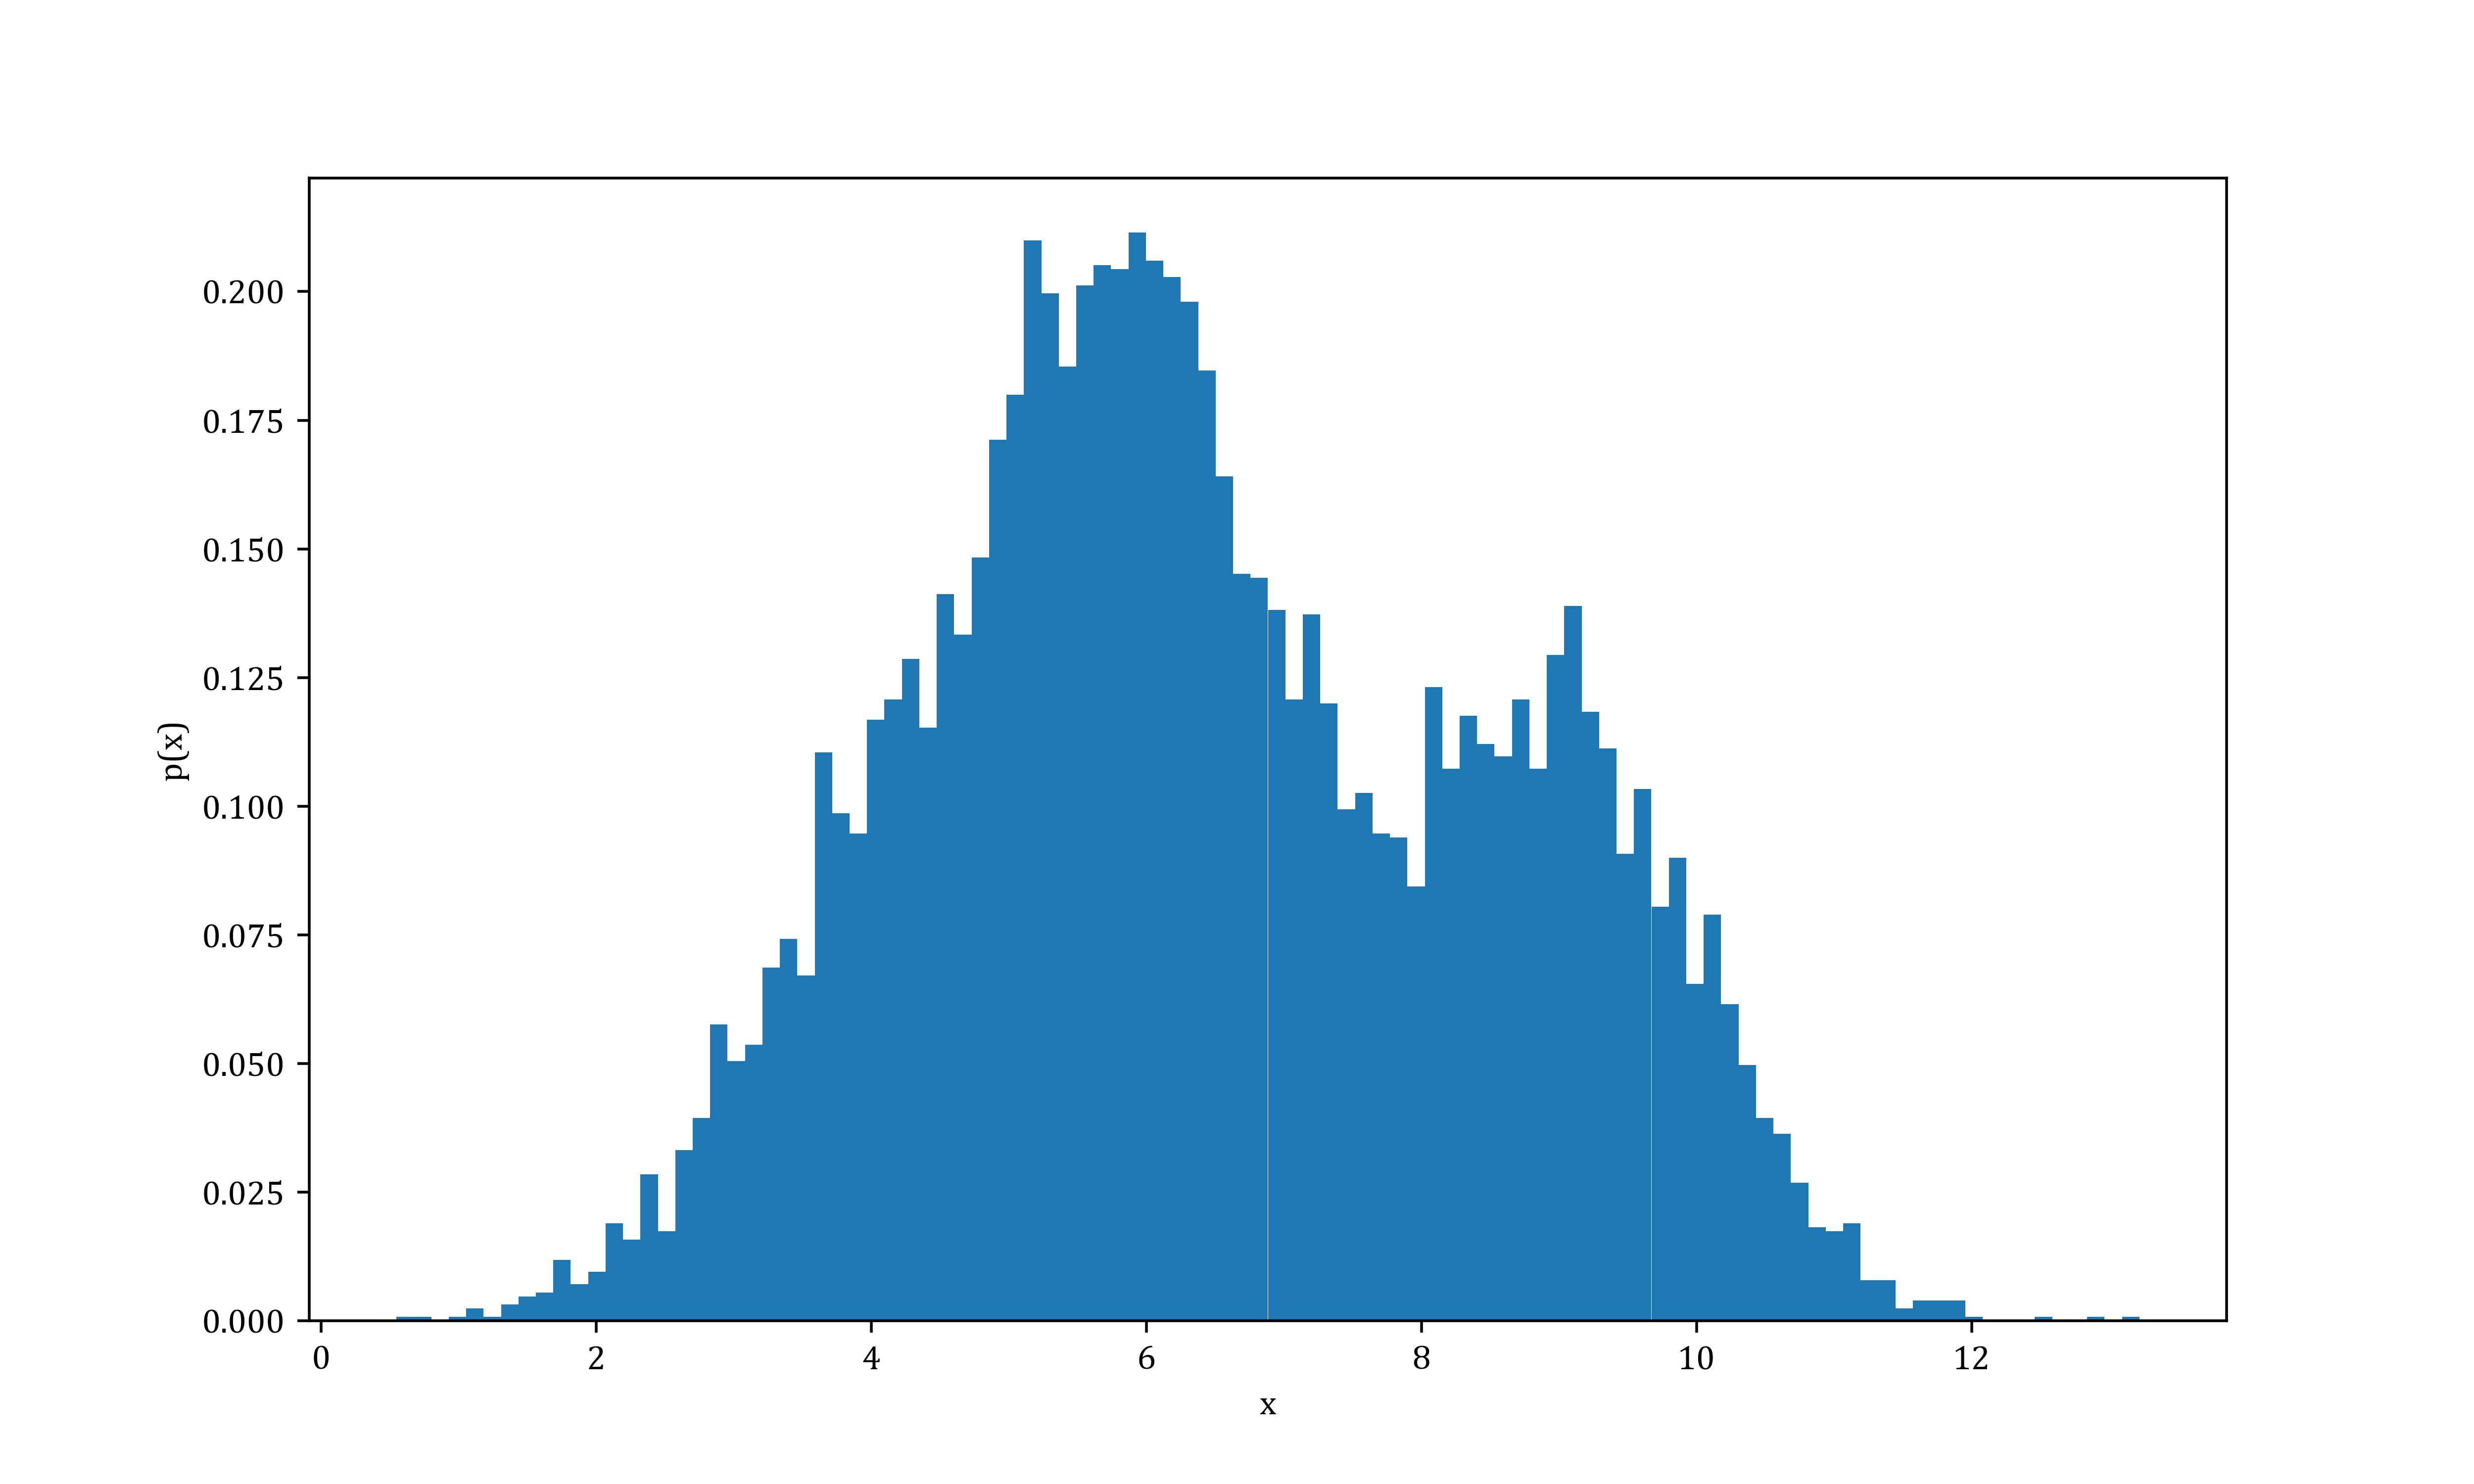
\includegraphics[width=0.8\textwidth]{assets/images/a3b.png}
    \caption{Histogram of the dataset}
    \label{fig_a3b}
\end{figure}

The code can be found in the \textbf{Task B} section in \texttt{code/3.ipynb}.

\section*{\colS{$\S$} Task C ($\star$) \hfill \normalfont \large [1+2+2]}

\begin{tcolorbox}
    We are still nowhere near finding a distribution that fits our data well.
    Let’s guess. It looks reasonably like a binomial distribution centered near
    about 6. Let us find the binomial distribution closest to our data.
    
    One way to define closeness is to ask for the first few moments to be equal
    (it is a theorem in statistics that if every moment of two distributions is
    identical, then the two distributions must be identical as well - we are
    roughly approximating this theorem here).

    In this task, we will find the best-fit binomial distribution to
    $\mathcal{D}$ by asking for the first two moments $\hat{\mu}_1$ and
    $\hat{\mu}_2$ to be equal to the corresponding two moments of $\text{Bin}(n,
    p)$, for some suitable choice of $n$ and $p$.

    (You need to estimate the mode, not the mean.)

    \vspace{10pt}
    \begin{enumerate}
        \item First, compute an expression for the first two moments $\mu^{Bin}_1,
        \mu^{Bin}_2$ of the distribution $\text{Bin}(n, p)$ as a function of $n$
        and $p$.
        \item Then, use the \texttt{fsolve} function from \texttt{scipy.optimize}
        to compute a solution $(n, p)$ to $\hat{\mu}_i = \mu^{Bin}_i, i = 1, 2$.
        Round $n$ to either $\floor{n}$ or $\ceil{n}$ based on which one
        satisfies the equalities better (they will not be exactly satisfied). Say
        the found parameters are $(n^*, p^*)$.
        \item Finally, using \texttt{numpy.linspace} and
        \texttt{scipy.stats.binom.pmf}, plot the binomial distribution $\text{Bin}
        (n^*, p^*)$ on top of the histogram of $\mathcal{D}$. It would help to get
        something like the figure in figure \ref{fig_q3c}.

        \begin{figure}[H]
            \centering
            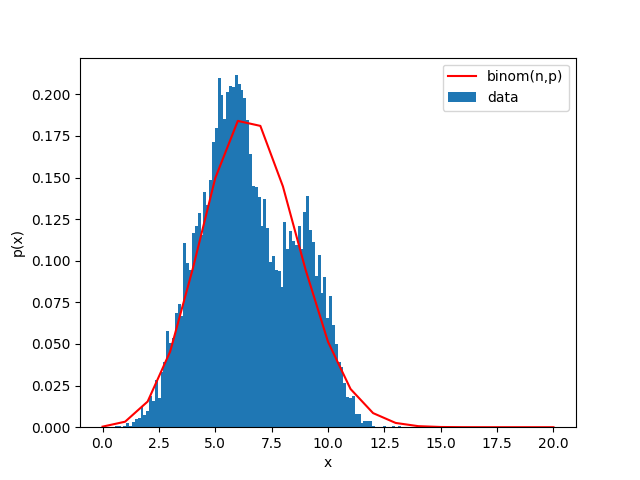
\includegraphics[width=0.5\textwidth]{assets/images/q3c.png}
            \caption{The best binomial distribution approximation to the true
            distribution}
            \label{fig_q3c}
        \end{figure}
    \end{enumerate}
\end{tcolorbox}

% Solution C

We will use the moment generating function
$M(t) = \sum_{n=0}^{\infty}P[X=n]e^{nt}$ to compute the expressions for the first
two moments of the distribution $\Bin(n, p)$. For the binomial distribution, the
PGF, as seen in \ref{e1.4} of Question 1, is
\begin{equation*}
    G(z) = (pz+1-p)^n.
\end{equation*}

Since $M(t)=G(e^t)$ by definition, we have

\begin{equation*}
    M(t) = (pe^t+1-p)^n.
\end{equation*}

Now, the two moments can be found using the relations $\mu_1^{\Bin}=M'(0)$ and
$\mu_2^{\Bin}=M''(0)$.

\begin{equation*}
    \begin{aligned}
        M'(t) &= n(pe^t+1-p)^{n-1}\cdot pe^t \\
        \implies M'(0) &= np \\
        \implies \mu_1^{\Bin} &= np.
    \end{aligned}
\end{equation*}

and for $n>1$,

\begin{equation*}
    \begin{aligned}
        M''(t) &= npe^t[(n-1)p(pe^t+1-p)^{n-2}+(pe^t+1-p)^{n-1}] \\
        \implies M''(0) &= np((n-1)p+1) \\
        \implies \mu_2^{\Bin} &= np((n-1)p+1) \\
        \implies \mu_2^{\Bin} &= np+n(n-1)p^2   
    \end{aligned}
\end{equation*}

The parameters for the best-fit binomial distribution were calculated using the
\texttt{scipy.optimize.fsolve} function. The parameters $(n^*, p^*)$ are:

\begin{equation*}
    (n^*, p^*) = (20, 0.32968652963757006).
\end{equation*}

The graph plotted can be found in \texttt{images/3c.png}.

It was plotted using \texttt{scipy.stats.binom.pmf} function,
\texttt{np.linspace} function and \texttt{matplotlib.pyplot}.

The plotted graph is at \ref{fig_a3c}.

\begin{figure}[H]
    \centering
    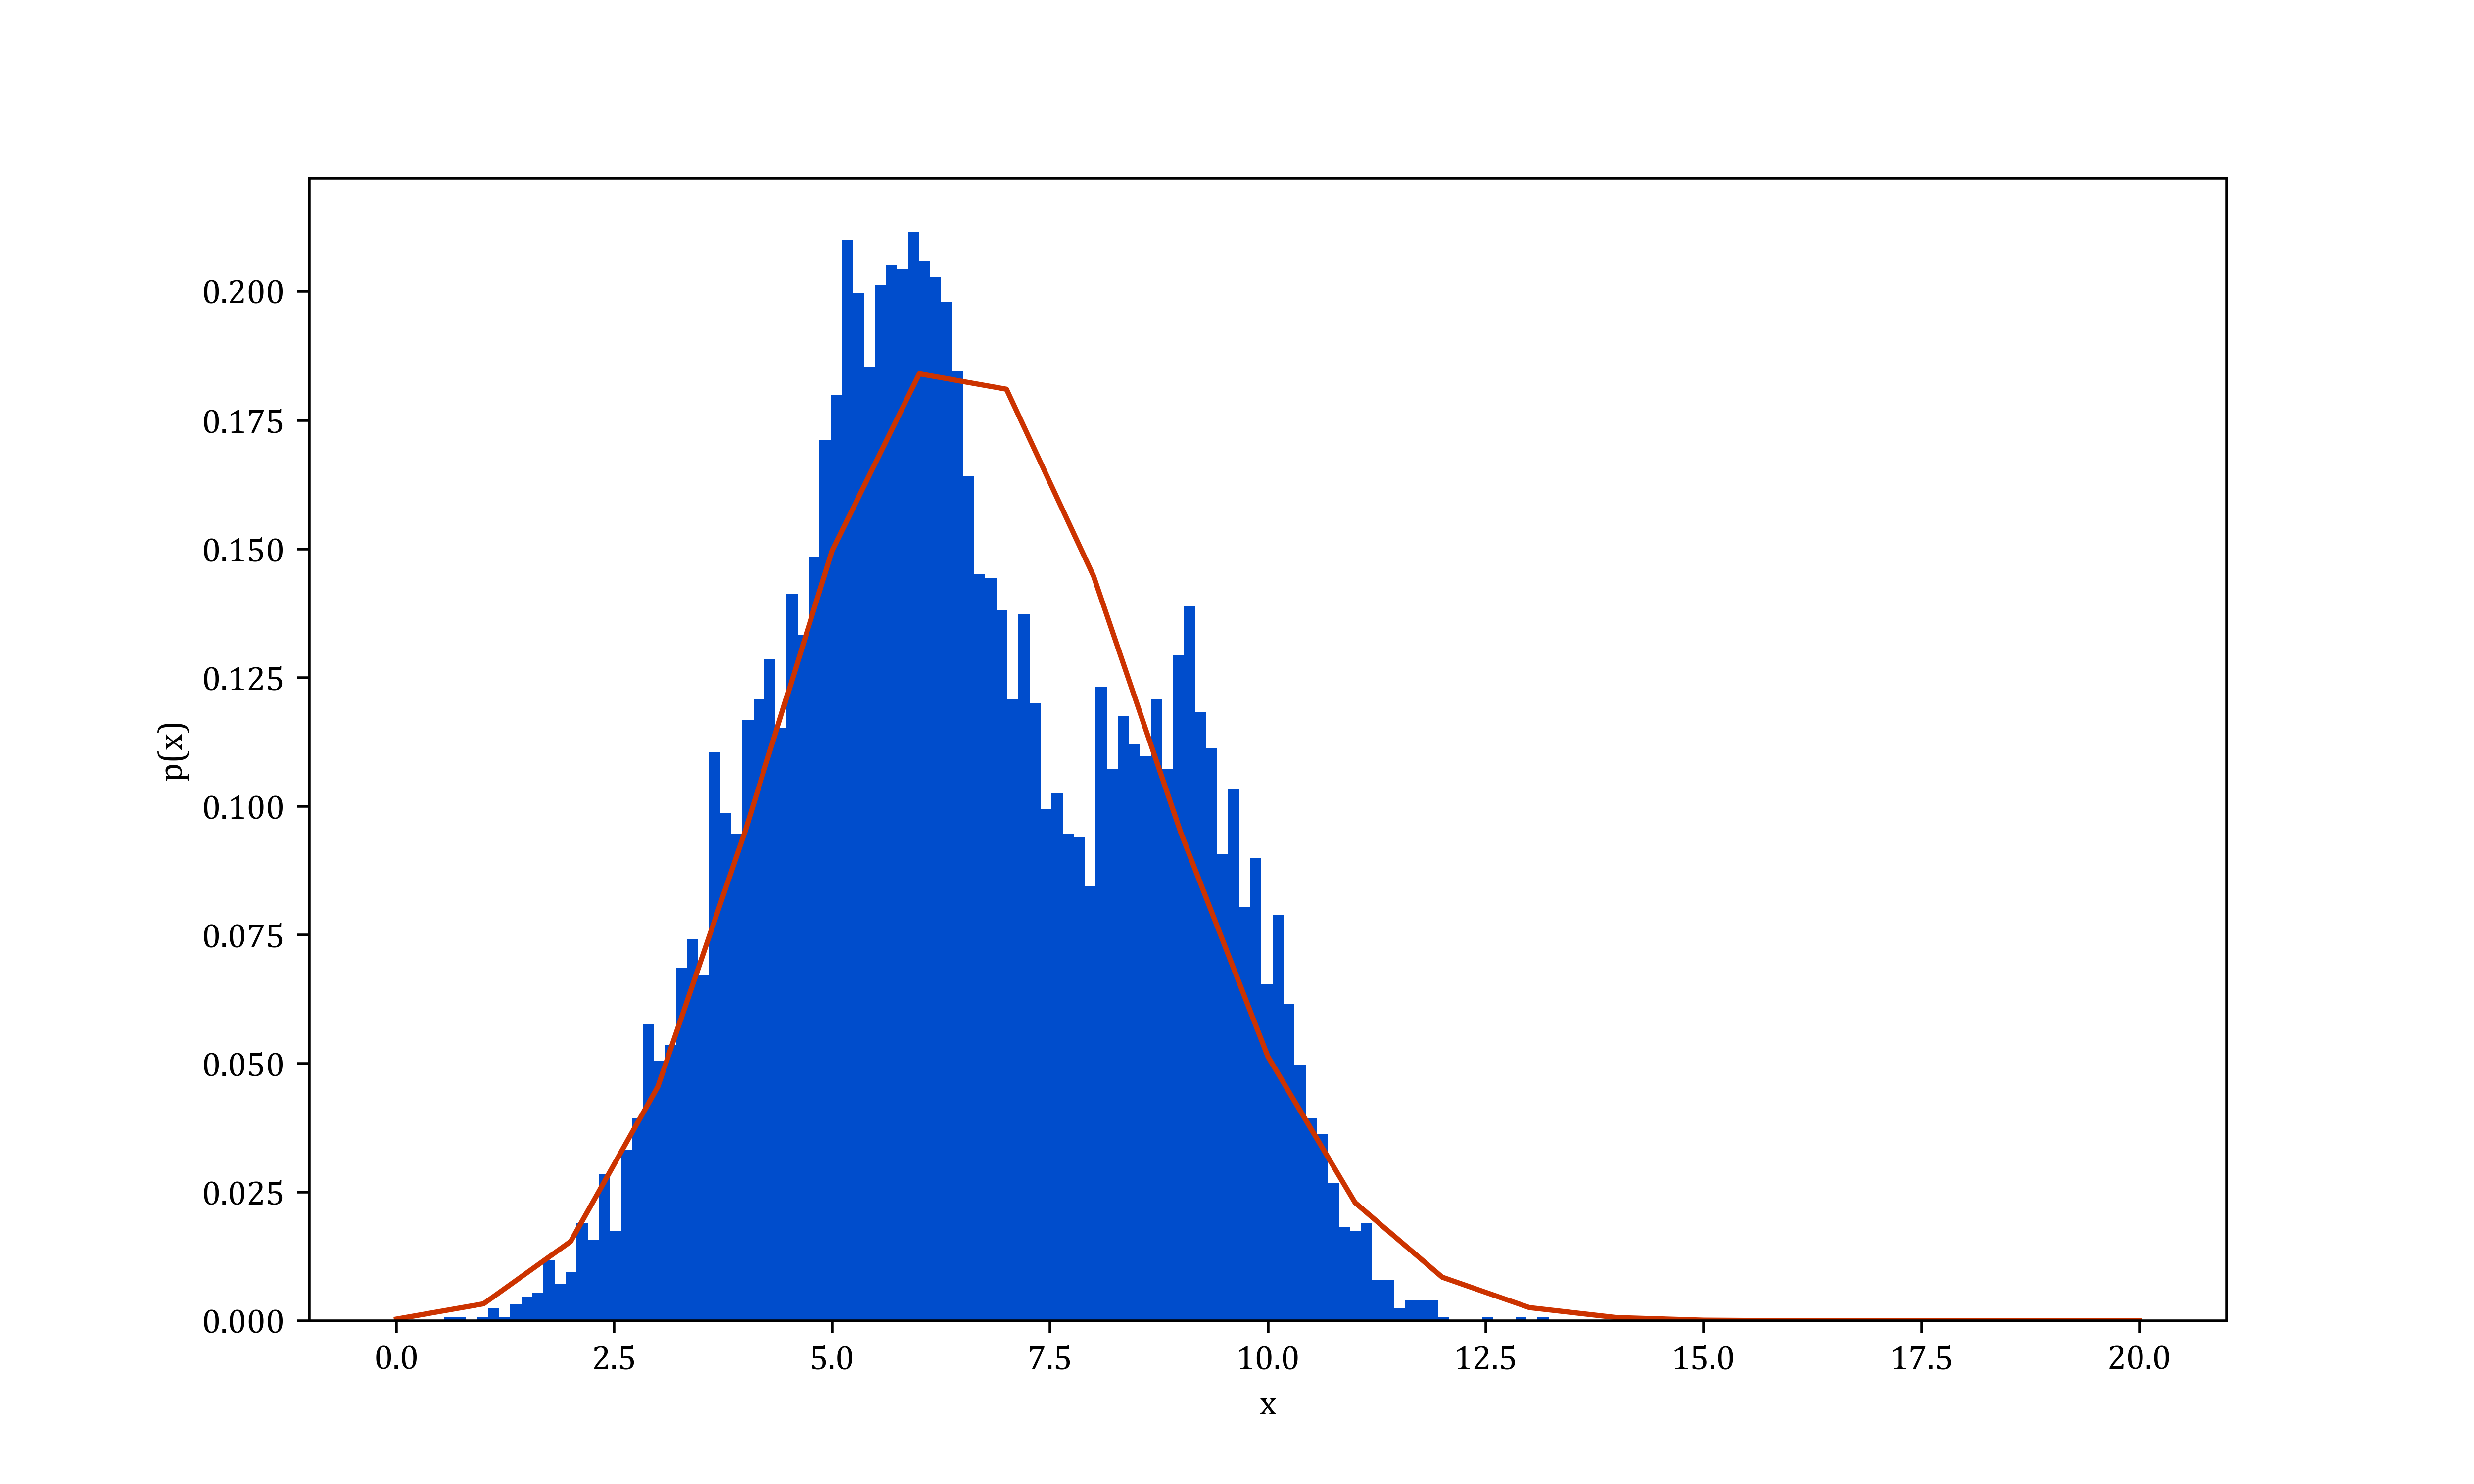
\includegraphics[width=0.8\textwidth]{assets/images/a3c.png}
    \caption{Binomial fit}
    \label{fig_a3c}
\end{figure}

The code can be found in the \textbf{Task C} section in \texttt{code/3.ipynb}.

\section*{\colS{$\S$} Task D \hfill \normalfont \large [3+2+2]}

\begin{tcolorbox}
    Well, that was not too bad an approximation. Let us try another distribution,
    which is continuous this time. The gamma distribution is a two-parameter
    family of continuous probability distributions. Two parameters parameterize
    it: shape parameter $k$ and scale parameter $\theta$/ Its probability density
    function is given by

    \begin{equation*}
        f(x; k, \theta) = \dfrac{1}{\theta^k \Gamma(k)} x^{k - 1} 
        e^{-\frac{x}{\theta}}
    \end{equation*}

    where $\Gamma(k) = \int_{0}^{\infty} t^{k - 1} e^{-t} dt$ is the Gamma
    function. We now wish to find the best Gamma-distribution approximation to the
    true distribution of $\mathcal{D}$.

    Your task and approach are essentially the same as in Task C. Restated for
    clarity, you must do the following:

    \vspace{10pt}
    \begin{enumerate}
        \item First, compute an expression for the first two moments
        $\mu_1^{\Gamma}, \mu_2^{\Gamma}$ of the distribution $\Gamma(k, \theta)$
        as a function of $k$ and $\theta$.
        \item Then, use the \texttt{fsolve} function from \texttt{scipy.optimize}
        to compute a solution $(k, \theta)$ to $\hat{\mu}_i = \mu^{\Gamma}_i, i =
        1, 2$. No rounding is required since $k$, $\theta$ may be real. The found
        parameters are $(k^*, \theta^*)$.
        \item Finally, using \texttt{numpy.linspace} and
        \texttt{scipy.stats.gamma.pdf} (the pdf takes three parameters: find out
        which ones are $k$ and $\theta$ and which one is 0), plot the binomial
        distribution $\text{Bin}(k^*, \theta^*)$ on top of the histogram of
        $\mathcal{D}$. It would help to get something like the figure in the
        figure \ref{fig_q3d}.
    
            \begin{figure}[H]
                \centering
                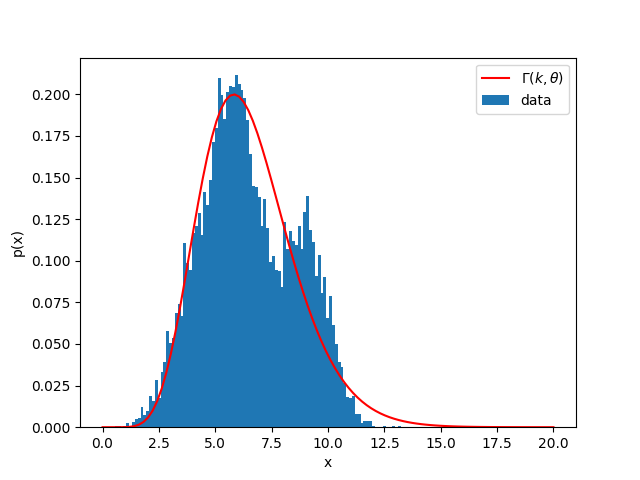
\includegraphics[width=0.5\textwidth]{assets/images/q3d.png}
                \caption{The best $\Gamma$ distribution approximation to the true
                distribution}
                \label{fig_q3d}
            \end{figure}
    \end{enumerate}
    
\end{tcolorbox}

% Solution D

We will first find the moment-generating function for the gamma distribution. Let
$x\sim \Gamma(k, \theta)$, then 
\begin{equation*}
    \begin{aligned}
        M(t) &= E[e^{tx}] \\
        &= \int_{-\infty}^{\infty}e^{tx}f(x; k, \theta)dx \\
        &= \int_{-\infty}^{\infty}e^{tx}
        \frac{1}{\theta^k\Gamma(k)}x^{k-1}e^{\frac{-x}{\theta}}dx.
    \end{aligned}
\end{equation*}

The first moment $\mu_1^{\Gamma}$ can be evaluated as $M'(0)$. Now

\begin{equation*}
    \begin{aligned}
        M'(t) &= \int_{-\infty}^{\infty}xe^{tx}
        \frac{1}{\theta^k\Gamma(k)}x^{k-1}e^{\frac{-x}{\theta}}dx.
    \end{aligned}
\end{equation*}

Substituting $\dfrac{x}{\theta}$ for $x$,

\begin{equation*}
    \begin{aligned}
        M'(t) &= \int_{-\infty}^{\infty}
        \frac{\theta}{\Gamma(k)}x^ke^{(t\theta-1)x}dx \\
        \implies M'(0) &= \int_{-\infty}^{\infty}
        \frac{\theta}{\Gamma(k)}x^ke^{-x}dx \\
        &= \frac{\theta}{\Gamma(k)}\int_{-\infty}^{\infty}k\cdot
        x^{k-1}e^{-x}dx \, \text{\ [using chain rule]}\\
        &= k\theta \\
        \implies \mu_1^{\Gamma} &= k\theta.
    \end{aligned}
\end{equation*}

Similarly, we will calculate the second moment $\mu_2^{\Gamma}$.

\begin{equation*}
    \begin{aligned}
        M''(t) &= \int_{-\infty}^{\infty}
        \frac{\theta}{\Gamma(k)}x^k\cdot \theta xe^{(t\theta-1)x}dx \\
        \implies M''(0) &= \int_{-\infty}^{\infty}
        \frac{\theta^2}{\Gamma(k)}x^{k+1}e^{-x}dx \\
        &= \frac{\theta^2}{\Gamma(k)}\int_{-\infty}^{\infty}(k+1)\cdot
        x^{k-1}e^{-x}dx \\
        &= k(k+1)\theta^2 \\
        \implies \mu_2^{\Gamma} &= k(k+1)\theta^2.
    \end{aligned}
\end{equation*}

The parameters for the best-fit gamma distribution were found to be

\begin{equation*}
    (k^*, \theta^*) = (9.691205541218757, 0.6703134703624737).
\end{equation*}

The equations were solved using \texttt{scipy.optimize.fsolve}.

The graph was plotted using \texttt{scipy.stats.gamma.pdf} function. The plot can
be found in \texttt{images/3d.png}.

The plotted graph is at \ref{fig_a3d}.

\begin{figure}[H]
    \centering
    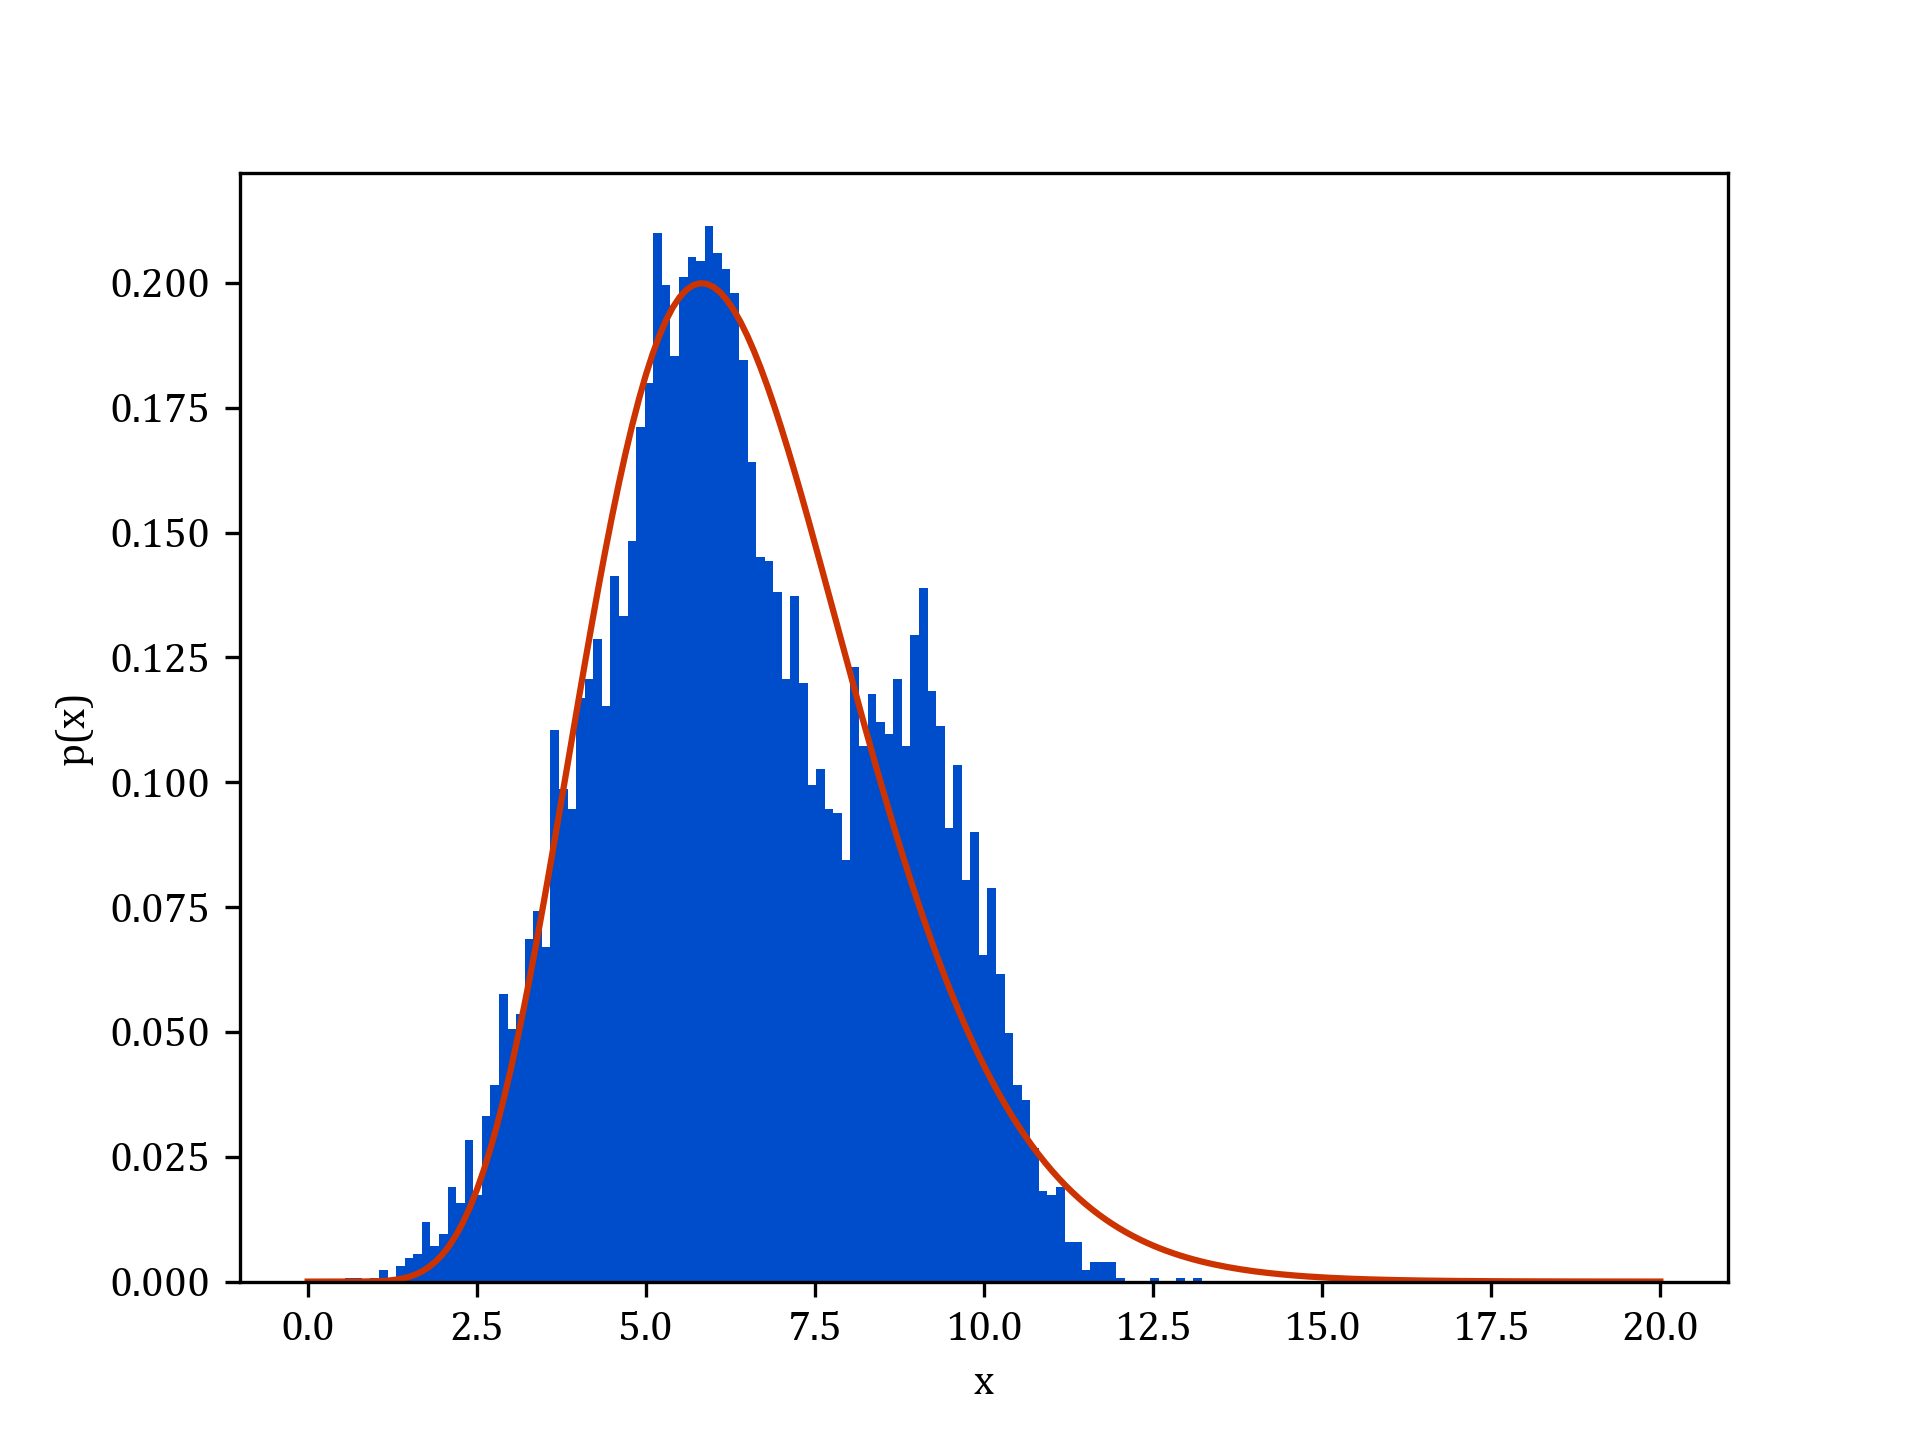
\includegraphics[width=0.8\textwidth]{assets/images/a3d.png}
    \caption{Gamma fit}
    \label{fig_a3d}
\end{figure}

The code can be found in the \textbf{Task D} section in \texttt{code/3.ipynb}.

\section*{\colS{$\S$} Task E ($\star$) \hfill \normalfont \large [3+3]}

\begin{tcolorbox}
    It looks like both of the distributions did a good job, but which one did a
    better job?
    
    A straightforward way to find out is to compute what is called the likelihood
    of the dataset. This is simply the probability that the dataset would
    $\mathcal{D}$, supposing that the actual distribution was our best-fit
    distribution.

    \vspace{10pt}
    \begin{mdframed}[backgroundcolor=lightblue, linecolor=blue, linewidth=1.5pt]
        \textbf{Definition 4 (Likelihood).}
        \textit{Given a dataset $S$ and a choice of parameter
        $\lambda = \lambda_0$ for a family of distributions $\text{P}[\lambda]$.
        Parameterized by $\lambda$, define the likelihood of $\lambda_0$ by}
        
        \begin{equation*}
           \mathcal{L}(\lambda_0 | S) := P_{\lambda_0}[S]
           = \prod_{i = 1}^{n} P_{\lambda_0}[X_i].
        \end{equation*}
    \end{mdframed}

    Here, $P_{\lambda_0}[x]$ is the PDF of the distribution whose parameter is
    $\lambda_0$. In our case, $P_{\lambda}[x]$ is
    $\text{Bin}(\lambda = (n, p))(x)$ or $\Gamma(\lambda = (n, p))(x)$.

    Since each probability is a small number for large datasets, the likelihood
    can underflow. Thus, the average log-likelihood is typically calculated:

    \begin{equation*}
        \ell(\theta | S) := \dfrac{\log{\mathcal{L}(\theta | S)}}{n},
    \end{equation*}

    where $n$ is the size of the dataset. Calculate (in code, no for loops
    allowed) the average log-likelihood for both best-fit distributions. Since
    $\text{Bin}(n, p)(x)$ is nonzero only at integer values of $x$. Before
    computing the likelihood, you must round each data point to the nearest 
    integer. No such thing is required for the Gamma distribution.
    
    A larger likelihood is typically attributed to a better fit. Which
    distribution was a better fit?
\end{tcolorbox}

% Solution E

The average log-likelihood for the best-fit binomial distribution is

\begin{equation}
    \ell((n, p)|\mathcal{D}) = -2.1570681154346785
\end{equation}

and the average log-likelihood for the best-fit gamma distribution is

\begin{equation}
    \ell((k, \theta)|\mathcal{D}) = -2.1608217722066647.
\end{equation}

The binomial distribution is a better fit.

\vspace{10pt}
The computation was done using \texttt{scipy.stats} module, and the
\texttt{numpy.log} \texttt{numpy.sum} functions.

The code used for calculating this is at code:\ref{code:3.2}.

\begin{lstlisting}[caption={Average log-likelihood}, label={code:3.2}]
# Average log-likelihood of binomial distribution
rnd = np.round(D)
probs = scipy.stats.binom.pmf(rnd, n, p)
L_bin = np.sum(np.log(probs)) / D.size
print("Avg. log-likelihood of binomial distribution:", L_bin)

# Average log-likelihood of gamma distribution
probs = scipy.stats.gamma.pdf(D, k, 0, theta)
L_gamma = np.sum(np.log(probs)) / D.size
print("Avg log-likelihood of gamma  distribution:", L_gamma)

# The binomial distribution was a better fit
\end{lstlisting}

The code can be found in the \textbf{Task E} section in \texttt{code/3.ipynb}.

\section*{\colS{$\S$} Task F \hfill \normalfont \large [2+2+2+2]}

\begin{tcolorbox}
    Notice the two peaks in the distribution? This immediately tells us that the
    distribution could not have been from a Binomial or Gamma function since those
    have a unique mode.
    
    A typical distribution with two peaks is the Gaussian Mixture Model, which is
    the subject of Question 5. Please read Task A of Question 5 before moving
    ahead.
    
    We will assume now that our distribution is composed of a two-component
    Gaussian mixture, each component having variance 1. That is, the distribution
    modeling of our data is assumed to have the pdf

    \begin{equation*}
        P[x] = \dfrac{1}{\sqrt{2\pi}}\left(
        p_1 \exp{\left(-\dfrac{(x - \mu_1)^2}{2}\right)} +
        p_2 \exp{\left(-\dfrac{(x - \mu_2)^2}{2}\right)}
        \right)
    \end{equation*}

    We have four parameters to find, and so we need four moments. To make things
    easy, here are the first four moments of this distribution (here $\sigma_1 =
    \sigma_2 = 1$):

    \begin{equation*}
        \begin{aligned}
            \mu_1^{\text{gmm}} &= p_1 \mu_1 + p_2 \mu_2. \\
            \mu_2^{\text{gmm}} &= p_1 (\sigma_1^2 + \mu_1^2) + p_2 (\sigma_2^2 +
            \mu_2^2).\\
            \mu_3^{\text{gmm}} &= p_1 (\mu_1^3 + 3 \mu_1 \sigma_1^2) + p_2
            (\mu_2^3 + 3 \mu_2 \sigma_2^2).\\
            \mu_4^{\text{gmm}} &= p_1 (\mu_1^4 + 6 \mu_1^2 \sigma_1^2 + 3
            \sigma_1^4) + p_2 (\mu_2^4 + 6 \mu_2^2 \sigma_2^2 + 3 \sigma_2^4).
        \end{aligned}
    \end{equation*}

    As in Tasks C and D, compute the following:

    \vspace{10pt}
    \begin{enumerate}
        \item First, compute $\hat{\mu}_i$ for  $i = 3, 4$.
        \item Then, use the \texttt{fsolve} function from \texttt{scipy.optimize}
        to compute a solution $(\mu_1, p_1, \mu_2, p_2)$ to $\hat{\mu}_i =
        \mu^{\text{gmm}}_i, i = 1, 2, 3, 4$. No rounding is required. Say the
        found parameters are $(\mu_1^*, p_1^*, \mu_2^*, p_2^*)$.
        \item Finally, using \texttt{numpy.linspace} and
        \texttt{scipy.stats.norm.pdf}, plot the GMM distribution obtained on top
        of the histogram of $\mathcal{D}$. You should get something like the
        figure in figure \ref{fig_q3f1}.
    \end{enumerate}

    \begin{figure}[H]
        \centering
        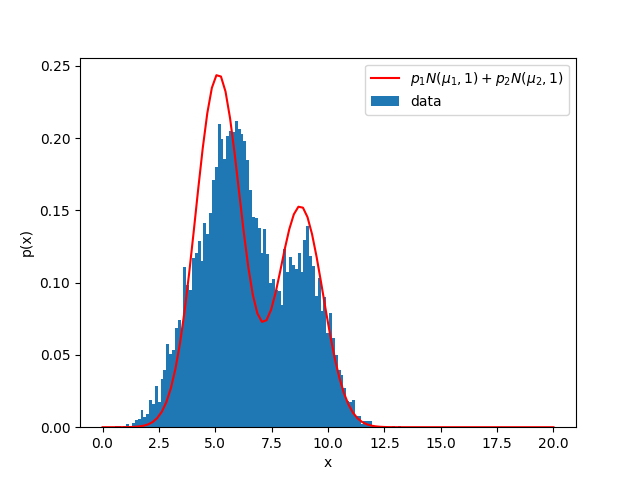
\includegraphics[width=0.5\textwidth]{assets/images/q3f1.png}
        \caption{The best two-component unit-variance GMM approximation to the
        true distribution}
        \label{fig_q3f1}
    \end{figure}

    To finish, compute the average negative log-likelihood of the obtained GMM
    distribution. Is it better an approximation than the previous two?
\end{tcolorbox}

% Solution F

The 3rd and 4th moments of $\mathcal{D}$, $\hat{\mu}_3$ and $\hat{\mu}_4$ are

\begin{equation*}
    \hat{\mu}_3 = 360.56586952543273
\end{equation*}

and

\begin{equation*}
    \hat{\mu}_4 = 2968.068491427333.
\end{equation*}

They can be calculated in a way similar to the one mentioned in \textbf{Task A}.

We have used a two-component Gaussian mixture, each component having variance 1.
The distribution is assumed to have the pdf:

\begin{equation*}
    P[x]=\frac{1}{\sqrtsign{2\pi}}\left(p_1\exp\left(-\frac
    {(x-\mu_1)^2}{2}\right)+p_2\exp\left(-\frac{(x-\mu_2)^2}{2}\right)\right).
\end{equation*}

The average negative log-likelihood of the best-fit GMM distribution is
\begin{equation*}
    -\ell((p_1, p_2, \mu_1, \mu_2)|\mathcal{D}) = 2.1830387449113133.
\end{equation*}

This turns out to be a worse approximation than the other two. Among the three
distributions seen till now, the binomial distribution is the best fit.

The plot can be found in \texttt{3f.png} and at \ref{fig_a3f}.

\begin{figure}[H]
    \centering
    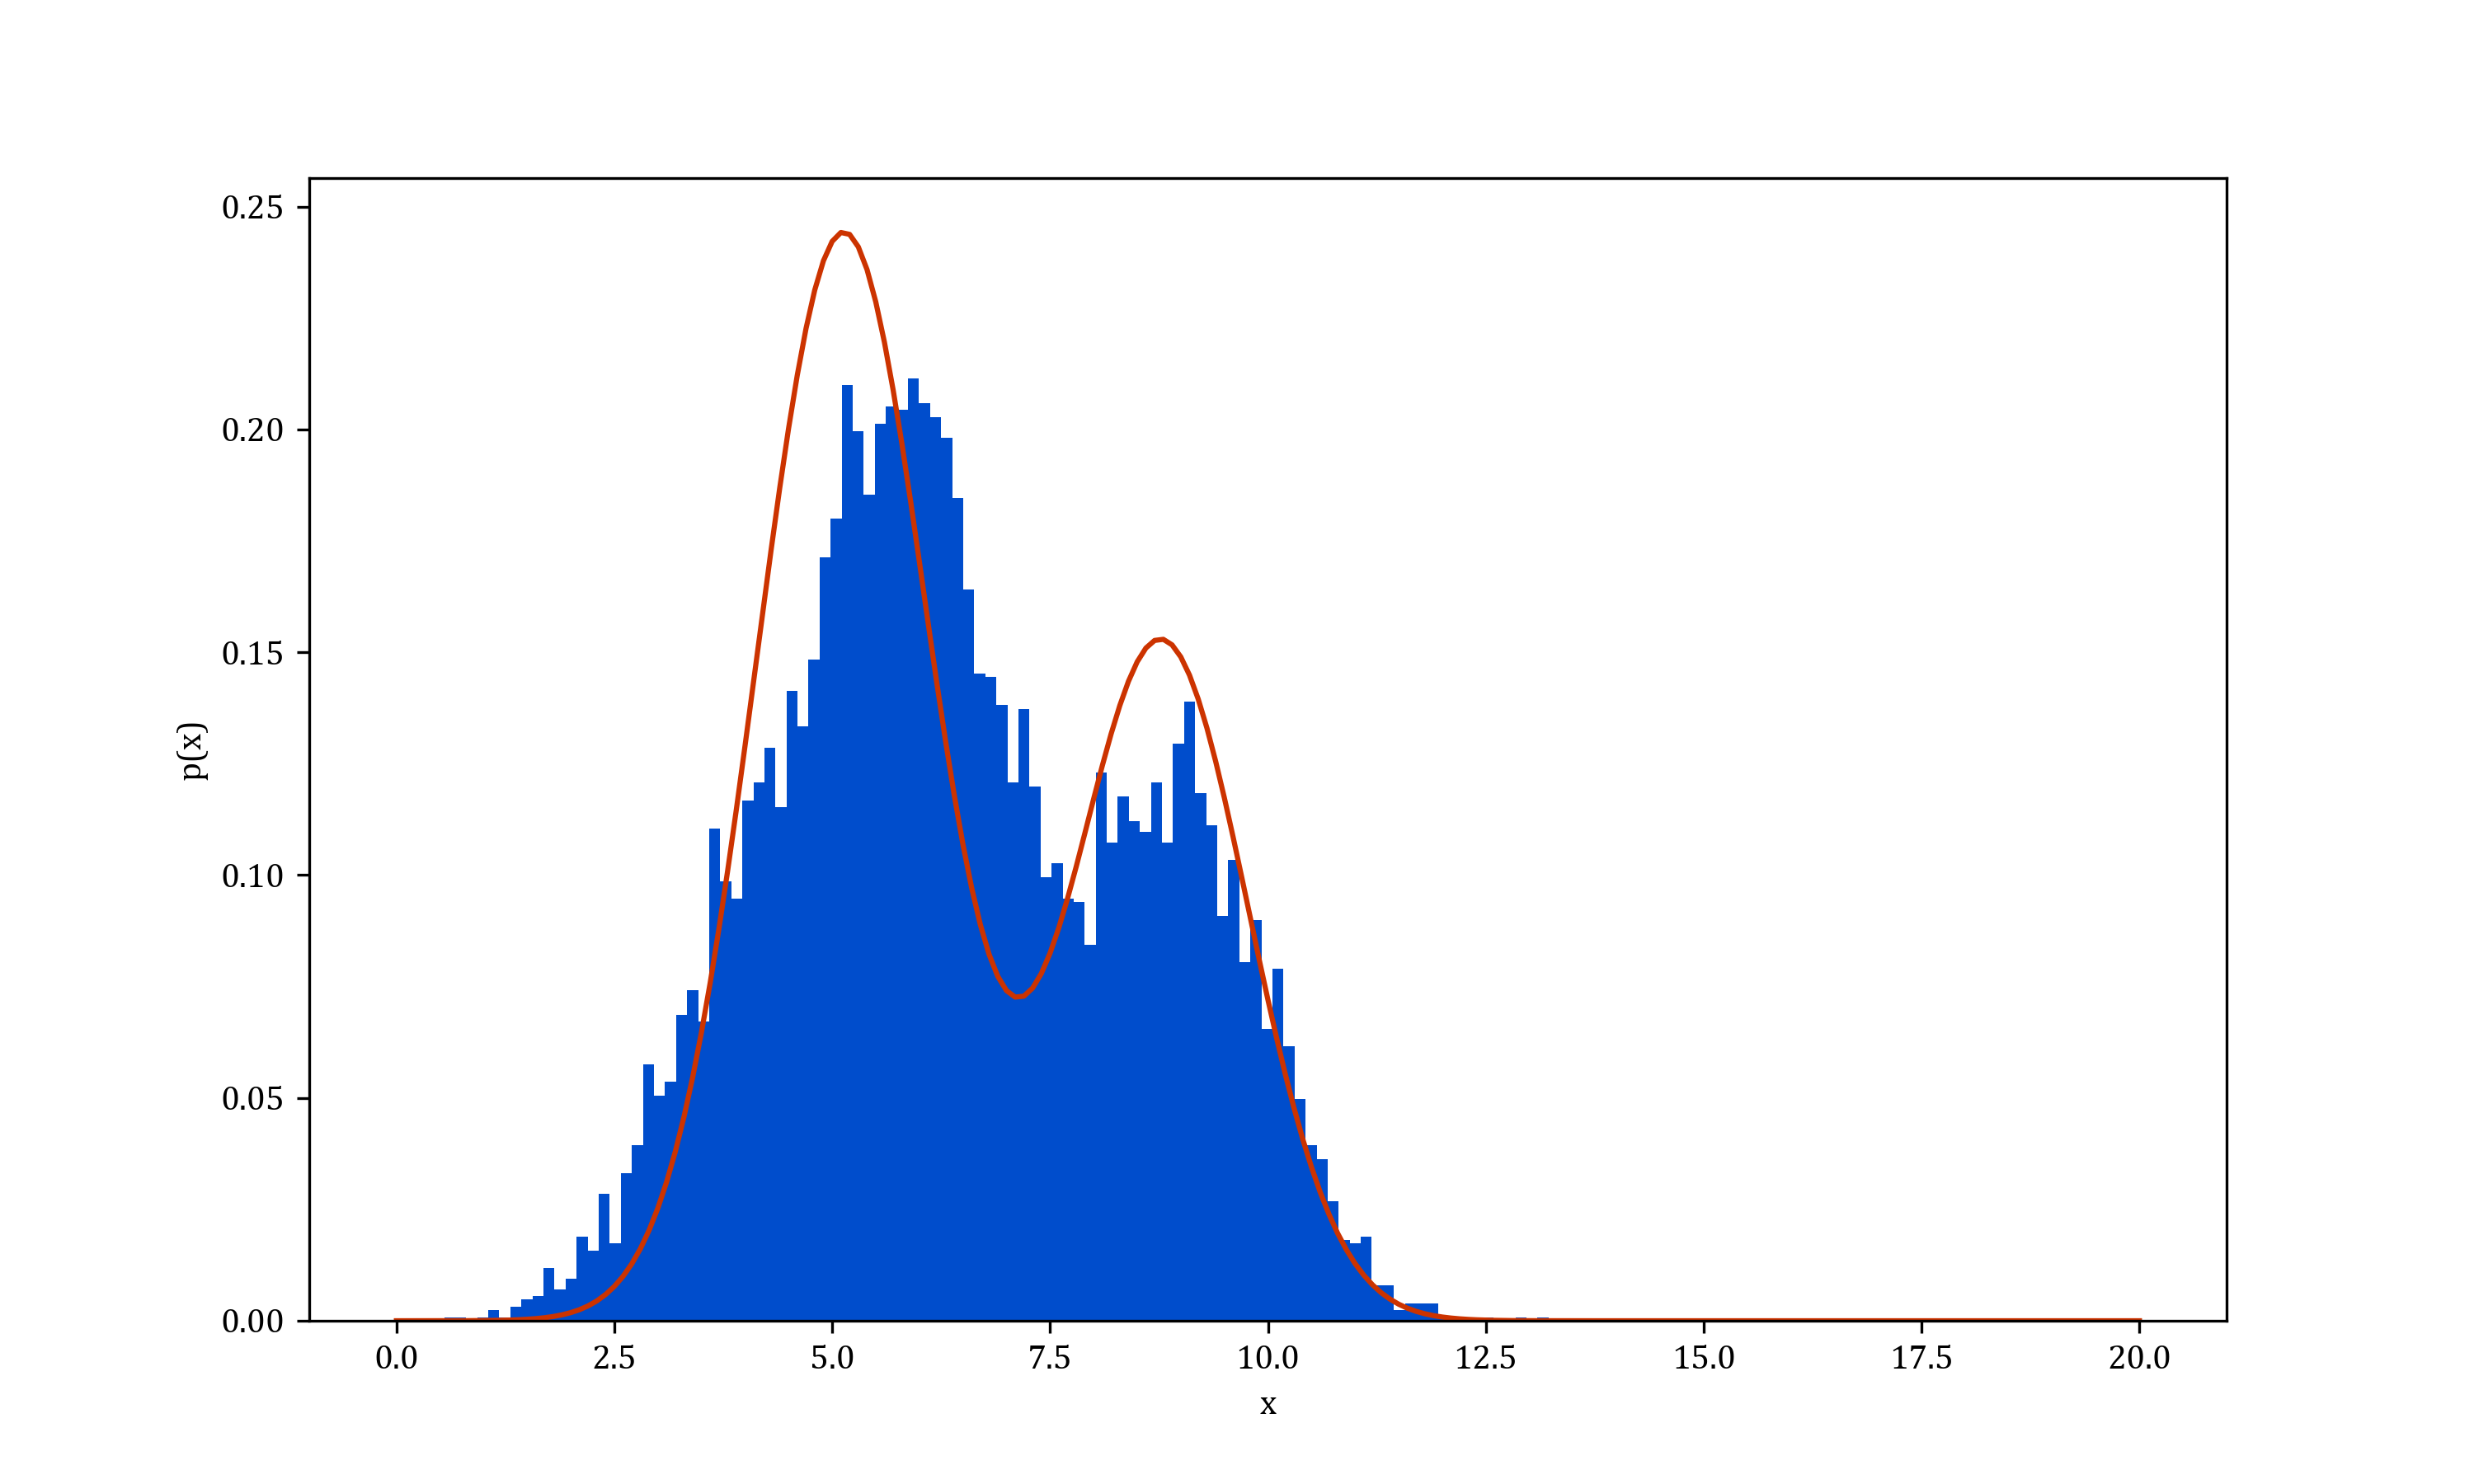
\includegraphics[width=0.8\textwidth]{assets/images/a3f.png}
    \caption{}
    \label{fig_a3f}
\end{figure}

\begin{tcolorbox}[title=]
    This task shows the power of a more versatile distribution like the GMM;
    indeed, clustering is typically done this way, using a GMM, the only
    difference being that an equation solver like \texttt{fsolve} is replaced by
    a heuristic called \textit{expectation maximization}, since solvers are slow
    for many-component GMMs.
\end{tcolorbox}

The code can be found in the \textbf{Task F} section in \texttt{code/3.ipynb}.

\section*{\colS{$\S$} Teaser}

\begin{tcolorbox}[title=]
    A different choice of distribution, with six parameters, gave the fit in the
    figure \ref{fig_q3f2}. An important part of machine learning is the parameter
    estimation to fit data. Feedforward neural networks typically do just that. As
    we have seen, more parameters can get you closer to the \enquote{right
    distribution}. It is not surprising that GPT has a few billion parameters that
    it learns. It is not just roses, though. A large number of parameters runs the
    risk of overfitting. Data Analysis and ML study better ways to learn parameter
    values, better families of distributions, how to detect and avoid overfitting,
    and more.

    \begin{figure}[H]
        \centering
        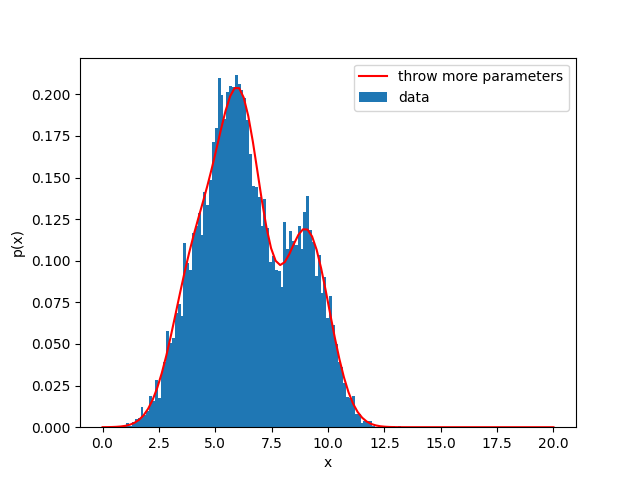
\includegraphics[width=0.5\textwidth]{assets/images/q3f2.png}
        \caption{Two more parameters bring the total to 6 parameters estimated
        using the first six moments}
        \label{fig_q3f2}
    \end{figure}
\end{tcolorbox}
    
\begin{tcolorbox}[title=Ungraded Bonus.]
    Can you guess what the true distribution is? Winners can claim a coffee treat
    at Cafe92 from the authors.
\end{tcolorbox}

% Solution: Ungraded Bonus.

The distribution which I got, to the closest of that curve is a 3 GMM.

I added what I got in the file \texttt{code/3.ipynb}.
